% A simple function under a positive graph, drawn as horizontal bands.
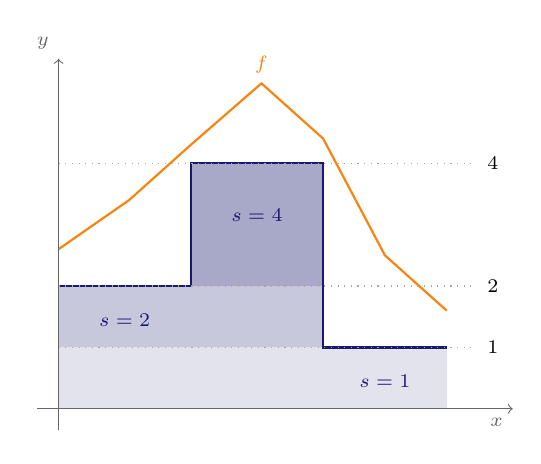
\begin{tikzpicture}[x=1.12cm,y=0.78cm]
  \fill[MidnightBlue!12] (0,0) rectangle (4.4,1);
  \fill[MidnightBlue!24] (0,1) rectangle (3.0,2);
  \fill[MidnightBlue!38] (1.5,2) rectangle (3.0,4);
  \draw[MidnightBlue,thick] (0,2) -- (1.5,2) -- (1.5,4) -- (3,4) -- (3,1) -- (4.4,1);
  \draw[BurntOrange,thick] (0,2.6) -- (0.8,3.4) -- (1.5,4.3) -- (2.3,5.3) -- (3.0,4.4) -- (3.7,2.5) -- (4.4,1.6);
  \draw[black!35,dotted] (0,1) -- (4.7,1);
  \draw[black!35,dotted] (0,2) -- (4.7,2);
  \draw[black!35,dotted] (0,4) -- (4.7,4);
  \node[font=\scriptsize,anchor=west] at (4.75,1) {$1$};
  \node[font=\scriptsize,anchor=west] at (4.75,2) {$2$};
  \node[font=\scriptsize,anchor=west] at (4.75,4) {$4$};
  \draw[->,black!60] (-0.25,0) -- (5.15,0) node[below left,font=\scriptsize] {$x$};
  \draw[->,black!60] (0,-0.35) -- (0,5.7) node[above left,font=\scriptsize] {$y$};
  \node[font=\scriptsize,MidnightBlue] at (0.75,1.45) {$s=2$};
  \node[font=\scriptsize,MidnightBlue] at (2.25,3.15) {$s=4$};
  \node[font=\scriptsize,MidnightBlue] at (3.7,0.45) {$s=1$};
  \node[font=\scriptsize,BurntOrange,anchor=south] at (2.3,5.3) {$f$};
\end{tikzpicture}
